\documentclass[twocolumn,11pt]{article}



\usepackage[margin=0.7in]{geometry}
\usepackage{authblk} % For author and affiliation blocks
\usepackage{tgpagella}
\setlength{\columnsep}{0.7in}
% --------------------------------------------------------
% Title and Author Configuration
% --------------------------------------------------------
\title{\textbf{Introduction to State Space Models (SSM)}}

\author[]{Vinay}
\author[]{Subhadeep Sing}
\author[]{Vaibhav Mahore}
\author[]{Snehal Biswas}


\affil[]{Indian Institute of Science, Bangalore \\
\texttt{\{vinay2023 ,shubadeeps ,mvaibhav ,snehalbiswas\}@iisc.ac.in}}




\date{October 26, 2020} % Customize or remove

% --------------------------------------------------------
% Begin Document
% --------------------------------------------------------
\begin{document}

\maketitle

\begin{abstract}
% Your abstract goes here.
This is a short abstract summarizing the paper. 
\end{abstract}

\section{Introduction}
% Your introduction goes here.
Sequential data modeling has emerged as a critical paradigm in modern machine learning and data analysis, addressing the fundamental challenge of processing and understanding information that unfolds over time or in a specific order. The inherent temporal dependencies and contextual relationships within sequential data present unique challenges that traditional static modeling approaches fail to adequately address. This limitation has driven significant research interest in developing specialized architectures and methodologies capable of capturing these temporal dynamics effectively. From natural language processing to financial forecasting, the applications of sequential data modeling span diverse domains, each presenting its own set of challenges and requirements. The evolution of sequential modeling techniques has witnessed several breakthrough developments, starting from simple Markov models to sophisticated neural architectures. Traditional feed-forward neural networks, while powerful for many tasks, proved inadequate for sequential data due to their inability to maintain state information across time steps. This limitation led to the development of recurrent neural networks (RNNs), which introduced the concept of memory through recurrent connections. However, RNNs themselves faced challenges with long-term dependencies, leading to the introduction of more sophisticated architectures like Long Short-Term Memory (LSTM) networks and Gated Recurrent Units (GRUs). These innovations marked significant progress in the field, enabling better handling of long-range dependencies and more stable training dynamics. Despite these advances, the quest for more efficient and effective sequential modeling approaches continues, driven by the ever-increasing complexity and scale of modern applications. The emergence of attention mechanisms and transformer architectures has further revolutionized the field, offering new perspectives on how to process sequential data more effectively.


\section{Related Work}
% Discuss related research, references, etc.

\section{Method}
% Detailed description of your proposed method or replication steps.

\section{Experiments}
% Describe experiments, datasets, metrics, etc.

\section{Conclusion}
% Conclude with key insights and future directions.

\bibliographystyle{abbrv}
\bibliography{references} % Or your .bib file

\end{document}



% lstm start from here
\documentclass[twocolumn,11pt]{article}

\usepackage[margin=0.7in]{geometry}
\usepackage{tgpagella}
\usepackage{graphicx}
\usepackage{amsmath}
\setlength{\columnsep}{0.7in}

\begin{document}

\section{\Large \textsc{LSTM: long short-term memory}}

In an RNN, it can easily predict the last word in “the clouds are in the sky” because no additional context is needed---it’s obvious that the next word is “sky.” However, consider a scenario like, “I grew up in France… I speak fluent \_\_\_\_\_\_.” In this case, the RNN fails to complete the sentence because it only has short-term memory and suffers from problems such as gradient explosion or vanishing gradients. Therefore, we need LSTM, an improved version of the RNN, to handle this type of problem. LSTMs overcome these issues by maintaining long-term memory, allowing them to use both short-term and long-term memory together. This combination enables more accurate predictions for tasks where context over longer sequences is crucial.

Now, let us explore the working principles of Long Short-Term Memory (LSTM) networks.

\begin{figure}[h!]
    \centering
    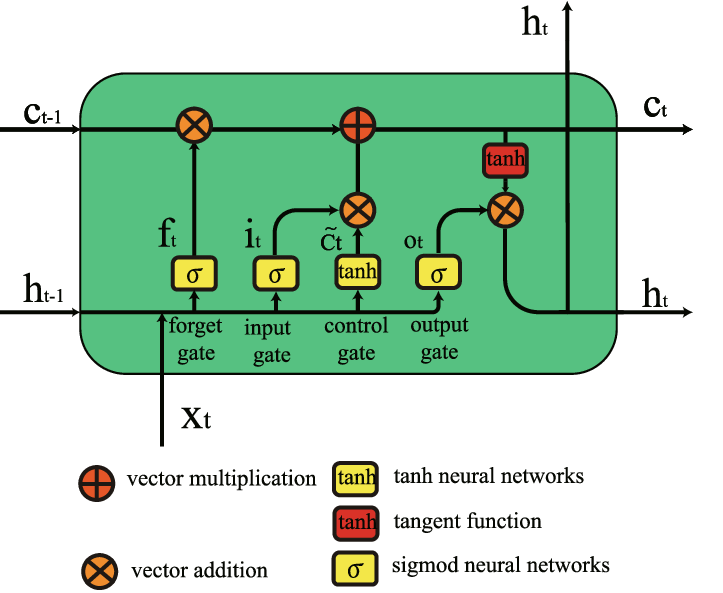
\includegraphics[scale=0.2]{LSTM.png} % Replace with your actual image file name
    \caption{LSTM Architecture}
    \label{fig:myimage}
\end{figure}

{\small
\[
\begin{aligned}
    f_t &= \sigma\bigl(W_f [h_{t-1}, x_t] + b_f\bigr),\\[5pt]
    i_t &= \sigma\bigl(W_i [h_{t-1}, x_t] + b_i\bigr),\\[5pt]
    \tilde{C}_t &= \tanh\bigl(W_C [h_{t-1}, x_t] + b_C\bigr),\\[5pt]
    C_t &= f_t \times C_{t-1} + i_t \times \tilde{C}_t,\\[5pt]
    o_t &= \sigma\bigl(W_o [h_{t-1}, x_t] + b_o\bigr),\\[5pt]
    h_t &= o_t \times \tanh\bigl(C_t\bigr).
\end{aligned}
\]
}

The core idea behind LSTM is the horizontal line running across the top of the diagram. It extends straight down the entire chain with only minor modifications, allowing information to flow along it unchanged.

The gates are designed to optionally permit information to pass through. They consist of sigmoid layer outputs that produce values between 0 and 1, indicating how much of each component should be allowed to pass.
{\small
\paragraph{Step 1: Forget Gate}
The forget gate decides which information to discard from the cell state. It takes the previous hidden state \(h_{t-1}\) and the current input \(x_t\) as input and outputs values between 0 and 1 for each component in \(C_{t-1}\):  
\[
f_t = \sigma\bigl(W_f [h_{t-1}, x_t] + b_f\bigr).
\]
}
{\small

\paragraph{Step 2: Input and Update}  
This step consists of two parts. First, the input gate, a sigmoid layer, decides which values to update:  
\[
i_t = \sigma\bigl(W_i [h_{t-1}, x_t] + b_i\bigr).
\]  
Next, a tanh layer generates candidate values \(\tilde{C}_t\) for updating the cell state:  
\[
\tilde{C}_t = \tanh\bigl(W_C [h_{t-1}, x_t] + b_C\bigr).
\]  
The new cell state is then computed by combining the previous state and the new candidate values:  
\[
C_t = f_t \times C_{t-1} + i_t \times \tilde{C}_t.
\]  
}
{\small
\paragraph{Step 3: Output Gate}
For the output, a sigmoid layer determines which parts of the cell state to emit:
\[
o_t = \sigma\bigl(W_o [h_{t-1}, x_t] + b_o\bigr).
\]
Then, the cell state \(C_t\) is passed through a tanh function (to constrain values between \(-1\) and \(1\)) and multiplied by \(o_t\) to obtain the new hidden state:
\[
h_t = o_t \times \tanh\bigl(C_t\bigr).
\]
}




\end{document}